\documentclass{article}[]
\usepackage{epsfig}
\usepackage{psfig}
\usepackage{graphicx}
\usepackage{url}
\usepackage{tikz}
\usetikzlibrary{matrix,chains,positioning,decorations.pathreplacing,arrows}
\begin{document}

\title{{\bf Credit risk prediction using Artificial Neural Network algorithm}\\ }

\author{Shruti Goyal\\ \vspace{0.4cm}\\ 
 16200726 \vspace{0.1cm}\\ MSc Business Analytics \vspace{0.1cm}\\ 
 UCD Michael Smurfit Graduate Business School}

\date{}
\maketitle
\begin{abstract}
  Artificial neural network is an information processing system which is influenced by human brain and works on the same principles of biological nervous system. They possess ability to extract meaning from complex and intricate data, by detecting trends and extracting patterns from it. This paper illustrates the ability of neural network model and linear regression model constructed to predict the creditworthiness of an application accurately and precisely with minimal false predictions and errors. The results are shown to be similar for both the models, thus, models are efficient to use depending on the type of application and attributes. \\
  \textbf{Keywords:} Credit Risk, Artificial Neural Network, Linear Regression
\end{abstract}

\section{Introduction}
\label{intro}
Credit risk or credit default indicates the probability of non-repayment of bank financial services that has been given to the customers. Credit risk has always been an extensively studied area in bank lending decisions. Credit risk plays a crucial role for banks and financial institutions, especially for commercial banks and it is always difficult to interpret and manage. Due to the advancements in technology, banks have managed to reduce the costs, in order to develop robust and sophisticated systems and models to predict and manage credit risk.
The objective of credit risk models is to evaluate the risk portfolio of the borrower and then assign a probability of default. Therefore, there has been a discussion on classification and discrimination problems for solving credit risk models \cite{pacelli2011artificial}. \\\\
Banks evaluate loan applications based on a subjective assessment made by the borrower. This assessment can lead to inefficient and inconsistent applications. Banks will be successful if they are able to reduce the credit risk and have a significant effect on economic growth of the country. In order to discriminate between good customers and bad customers, banks developed a need for a model-based approach that can predict credit default accurately. The model-based approach provides better credit default management and efficiently allocate capital \cite{angelini2008neural}. \\\\
To predict the credit default, several methods have been created and proposed. The use of method depends on the complexity of banks and financial instituions, size and type of the loan. The commonly used method has been discrimination analysis. This method uses a score function that helps in decision making whereas some researchers have stated doubts on the validity of discriminates analysis because of its restrictive assumptions; normality and independence among variables \cite{eisenbeis1977pitfalls}. Artificial neural network models have created to overcome the shortcomings of other inefficient credit default models.\\\\
The objective of this paper is to study the ability of neural network algorithms to tackle the problem of predicting credit default, that measures the creditworthiness of the loan application over a time period. Feed forward neural network algorithm is applied to a small dataset of residential mortgages applications of a bank to predict the credit default. The output of the model will generate a binary value that can be used as a classifier that will help banks to identify whether the borrower will default or not default. This paper will follow an empirical approach which will discuss two neural network based models and experimental results will be reported by training and validating the models on residential mortgage loan applications. As the final step in the direction, linear regression method is also performed on the dataset. Results will provide a comparison between the efficiency and accuracy of the neural network and linear regression methods. As the paper follows an empirical approach, this paper will show structured experimental approach to the design of models. 

\section{Artificial Neural Network}
Discriminant analysis method has been the most common method to build credit default or credit score models. Although, this linear methodology has been criticized by the researchers because of its assumptions on the categorical data and unequal covariance matrices of good and bad customer loans.\\\\
An artificial neural network \cite{hornik1989multilayer}\cite{bebis1994feed} is a nonlinear approach that provides a new alternative to linear methods, especially in the situations where the dataset possess complex relationships between the independence of the nonlinear variables \cite{atiya2001bankruptcy} \cite{pang2002credit}. Artificial neural network is a learning system that models a relationship between inputs and outputs, taking into account the relationship is nonlinear. They are also known as black box systems, in which extraction of information from internal system is impossible \cite{angelini2008neural}.\\\\
Artificial Neural networks are machine learning system that simulates structure and function similar to a biological neuron. ANNs perform a task by changing its parameters, the same way a neuron changes its states to perform a cognitive task. A network is composed of a set of neurons structured in a specified topology. Neurons are connected by links with associated weights which determines information flow intensity; weights are the functions that represent behavior of the neural network.\\\\
\begin{figure}[!htb]
\centering
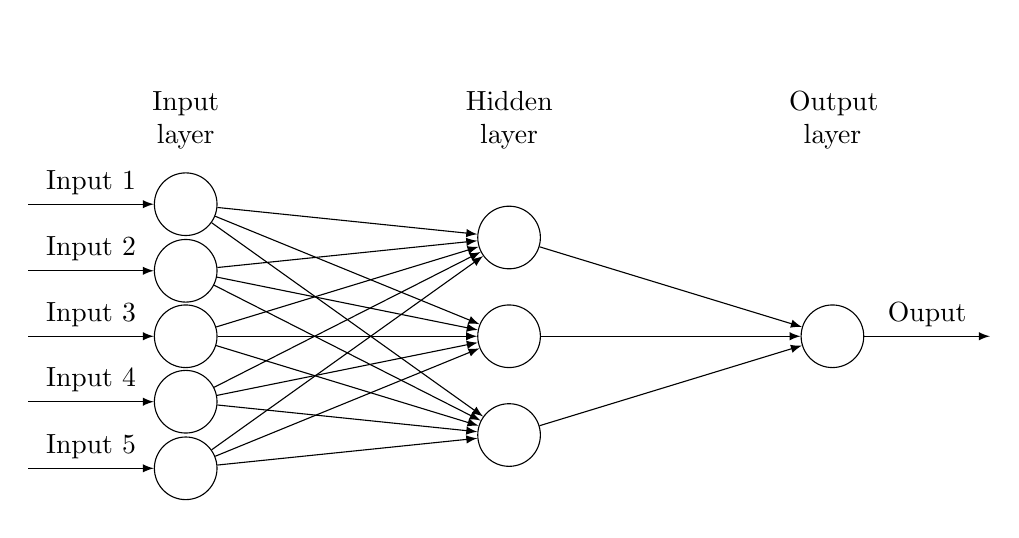
\begin{tikzpicture}[
plain/.style={
  draw=none,
  fill=none,
  },
net/.style={
  matrix of nodes,
  nodes={
    draw,
    circle,
    inner sep=8pt
    },
  nodes in empty cells,
  column sep=2cm,
  row sep=-11pt
  },
>=latex
]
\matrix[net] (mat)
{
|[plain]| \parbox{1.1cm}{\centering Input\\layer} & |[plain]| \parbox{1.1cm}{\centering Hidden\\layer} & |[plain]| \parbox{1.1cm}{\centering Output\\layer} \\
& |[plain]| \\
|[plain]| & \\
& |[plain]| \\
  |[plain]| & |[plain]| \\
& & \\
  |[plain]| & |[plain]| \\
& |[plain]| \\
  |[plain]| & \\
& |[plain]| \\    };
\foreach \ai [count=\mi ]in {2,4,...,10}
  \draw[<-] (mat-\ai-1) -- node[above] {Input \mi} +(-2cm,0);
\foreach \ai in {2,4,...,10}
{\foreach \aii in {3,6,9}
  \draw[->] (mat-\ai-1) -- (mat-\aii-2);
}
\foreach \ai in {3,6,9}
  \draw[->] (mat-\ai-2) -- (mat-6-3);
\draw[->] (mat-6-3) -- node[above] {Ouput} +(2cm,0);
\end{tikzpicture}
\caption{Basic Structure of Artificial Neural Network}
\label{fig:ANN1}
\end{figure}
As shown in figure \ref{fig:ANN1}, ANN has three layers, input layer, a hidden layer and output layer, input layer represents neurons receiving input stimulus. Then the information is transferred to next level of layer known as a hidden layer. Information is weighed before sending to next level of layers depending upon the size of the connections amongst neurons. Information is sized as per the processing unit or a transfer function represented in figure \ref{fig:ANN2}.\\
\begin{figure}[!htb]
\centering
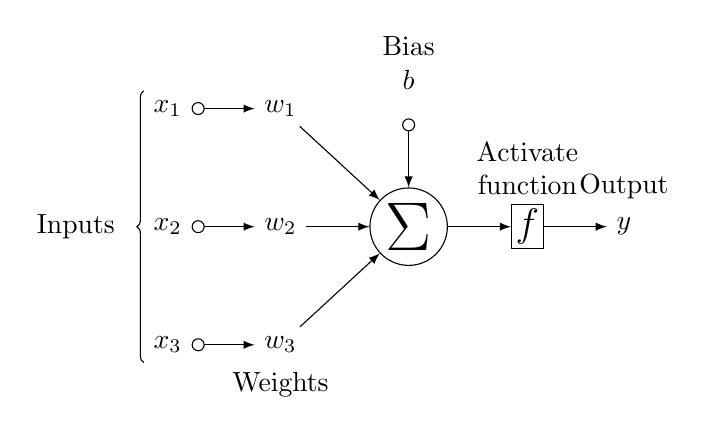
\begin{tikzpicture}[
init/.style={
  draw,
  circle,
  inner sep=1.5pt,
  font=\Huge,
  join = by -latex
},
squa/.style={
  draw,
  inner sep=1.5pt,
  font=\Large,
  join = by -latex
},
start chain=2,node distance=8mm
]
\node[on chain=2] 
  (x2) {$x_2$};
\node[on chain=2,join=by o-latex] 
  {$w_2$};
\node[on chain=2,init] (sigma) 
  {$\displaystyle\Sigma$};
\node[on chain=2,squa,label=above:{\parbox{1.5cm}{\centering Activate \\ function}}]   
  {$f$};
\node[on chain=2,label=above:Output,join=by -latex] 
  {$y$};
\begin{scope}[start chain=1]
\node[on chain=1] at (0,1.5cm) 
  (x1) {$x_1$};
\node[on chain=1,join=by o-latex] 
  (w1) {$w_1$};
\end{scope}
\begin{scope}[start chain=3]
\node[on chain=3] at (0,-1.5cm) 
  (x3) {$x_3$};
\node[on chain=3,label=below:Weights,join=by o-latex] 
  (w3) {$w_3$};
\end{scope}
\node[label=above:\parbox{2cm}{\centering Bias \\ $b$}] at (sigma|-w1) (b) {};

\draw[-latex] (w1) -- (sigma);
\draw[-latex] (w3) -- (sigma);
\draw[o-latex] (b) -- (sigma);

\draw[decorate,decoration={brace,mirror}] (x1.north west) -- node[left=7pt] {Inputs} (x3.south west);
\end{tikzpicture}
\caption{Mathematical Equation of Artificial Neural Network}
\label{fig:ANN2}
\end{figure}
Each neuron is characterized by a minimum value that activates a neuron(threshold value) and a transfer function. A Hidden layer can consist of several layers and performs the summation of input neurons and multiplies the weights with the summation to generate output neurons. Output generation is a two-step process: first, each input is multiplied by the weight on corresponding connection and then all valued are summed together; second, activation function is applied to summation of the inputs \cite{angelini2008neural}.\\
\begin{equation}
y_{i} = \sum_{j \in I} W_{j,i}a_{j}
\label{eq:1}
\end{equation}

\begin{equation}
a_{i} = g(y)    
\label{eq:2}
\end{equation}

Equation \ref{eq:1} represents evaluation of input and \ref{eq:2} represents activation function; where $W_{j,i}$ represents weights on the connection between $j$ and $i$ and $a_{j}$ is activation function of neuron $j$.\\\\
For a neural network to work efficiently, weights should be tuned accurately. This task can be achieved by using a learning algorithm, which trains the network and modifies weights until verified. Mostly, these algorithms stop when there occurs an error between output generated by network falls under threshold and expected output. There are three types of learning algorithms for artificial neural networks \cite{angelini2008neural}:
\begin{enumerate}
\item Supervised Learning
\item Unsupervised Learning
\item Reinforced Learning
\end{enumerate}

In supervised learning, a training set of correct examples is being used to train the network model. It consists of pairs of several inputs and expected outputs. Weights will be tuned based on the errors generated in the network. Most common example of supervised learning is classification, where the network has to learn to generalize relations between corresponding input and output variables. In this paper, we will be dealing with the typical classification problem to predict the credit default. 

\section{Methodology}
\subsection{Data}
Data has been collected from kaggle.com (lending club loan data) that consists of more than 8.5 million records. A random sample data of 60,000 records has been extracted from the dataset and appropriate attribute selection has been done from 80 attributes. Attribute selection includes numeric and integer attributes along with some factor attributes relevant to the problem this paper is dealing with. Dataset consists of dependent and independent variables as follows: 
\begin{enumerate}
\item \textbf{Dependent Variable:} loan\_status(0 and 1); this paper aims to predict the creditworthiness of the borrower in near future. In this context, if the borrower will default then the investment will be bad and if the borrower will not default then he or she will be able to repay the full loan amount. So, to differentiate in neural network 0 indicates borrower will default and 1 indicates borrower will not default.
\item \textbf{Independent Variable:} Following variables are considered as independent variable:
\begin{enumerate}
\item loan\_amnt: Amount of the loan that has been given to the borrower and in case of probationary loans, amount can be reduced in future
\item funded\_amnt: Amount that has been asked by the borrower to loan at beginning
\item funded\_amnt\_inv: Amount that has been committed by the investors
\item term: Total period that has been agreed upon to repay the loan
\item int\_rate: Interest rate on which loan has been given
\item installment: Amount agreed to repay the loan monthly
\item grade: Credit rating assigned to the loan application
\item emp\_length: Total number of years the borrower has been employed
\item annual\_inc: Annual income reported by the borrower while filing an application 
\item issue\_d: Issued date of the loan application
\item application\_type: Whether the application is individual or joint
\end{enumerate} 
\end{enumerate}

\subsection{Model}
In this study, a classic feed forward neural network has been used. The feedforward network consists of an input layer with 10 input variables, 7 hidden layer and an output layer with one neuron that represents a classifier. The network is trained by using a supervised learning algorithm(back propagation algorithm \cite{hecht1988theory}\cite{pineda1987generalization}). The algorithm optimise the neuron weights be minimising the error between actual and desired output. Error is $error_{i}$ $= D_{i} - A_{i}$ for neuron $i$. Weights will be updated by formula $W_{i,k} = W_{i,k} + \phi I_{k}error_{i}g^{'}(in_{i})$, where $\phi$ be the learning coefficient and $I_{k}$ is the output from hidden layer. Algorithm will work until a stopping criteria is found.\\\\
It is necessary to carefully choose the parameters, such as value of $\phi$ and number of neurons and number of hidden layers, for the neural network algorithm as shown in figure \ref{fig:nn}. In \ref{fig:nn} connections are represented by black lines between every layer and weights and blue line shows the bias(intercept of model) in every step. Network is black box and training algorithm is ready to use as it is converged.  Also, a random sample has been created from the extracted dataset for the network algorithm. Then a training and test dataset are created used to train the model and to validate the performance of the model respectively.\\\\ 
\begin{figure}[!htb]
\centering
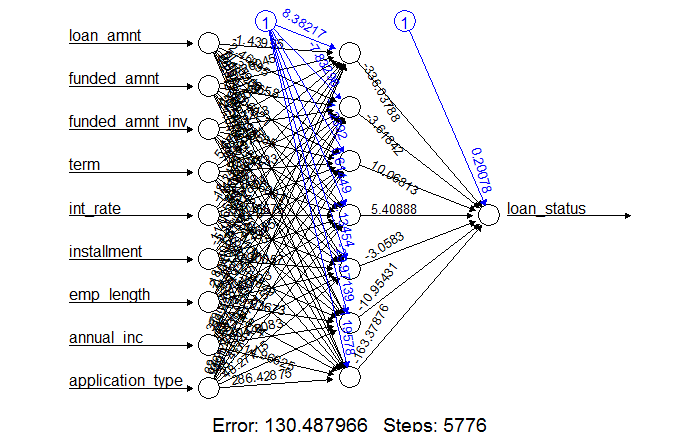
\includegraphics[width=1\textwidth]{nn.png}
\caption{Neural network plot of the credit default model}
\label{fig:nn}
\end{figure}
Also, to keep in mind that useless fields will be erased from the dataset, such that neural network will only work on numeric and integer variables. Next, data normalization is performed to feed the neural network with data that ranges in same interval. Min and max linear transformation function has been used to normalise the data before splitting the dataset into training and test datasets. 

\section{Experiments and Results}
There are $10$ normalized variables have been fed as the input to the network arranged in an order. Output of the network is a classifier that results in $0$ and $1$. At first, data has been checked for missing datapoint value, no data was missing; there was no need to fix the dataset. Correlation matrix of the inputs have been shown in figure \ref{fig:image1}.
\begin{figure}[!htb]
\centering
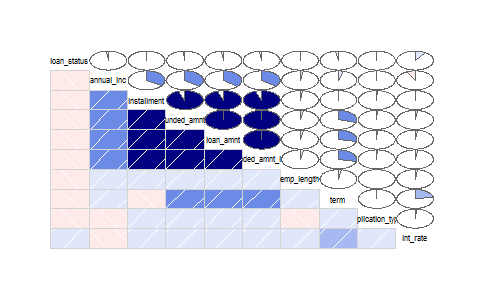
\includegraphics[width=1\textwidth]{image2.png}
\caption{Correlation Plot of the input dataset}
\label{fig:image1}
\end{figure}\\\\
Once the dataset was trained, it was tested on the test dataset. To compute the output based on the other inputs, \textbf{compute} function has been used. $7$ hidden layers were added to the network and model was created. Following result matrix has been generated by the network:
\begin{table} 
\caption{Result matrix for classic feed forward neural network} % title of Table 
\centering      % used for centering table 
\begin{tabular}{l|c}  % centered columns
\hline                      %inserts double horizontal lines 
{\bf Attribute}&{\bf Value}\\
%heading 
\hline                    % inserts single horizontal line 
Error & 322.833\\
Reached Threshold & 0.0998\\
Steps & 6765\\
\hline     %inserts single line 
\end{tabular} 
\label{table:params} 
\end{table} \\\\
Total $6765$ steps were needed until all derivatives of the error function  was smaller than default threshold($0.01$). After implementing classic feed forward algorithm, another model has been implemented by using back propagation algorithm with $0.01$ learning rate. Classic process and back propagation process have almost same error rate. Thus, classic model fit is less satisfied than back propagation algorithm.\\\\
\begin{figure}[!htb]
\centering
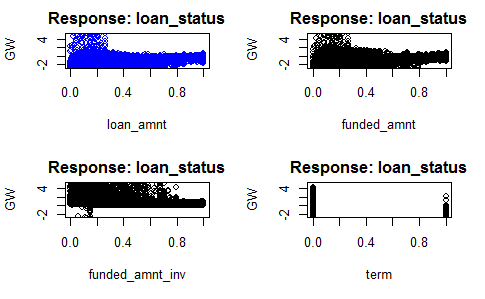
\includegraphics[width=0.8\textwidth]{image3.png}
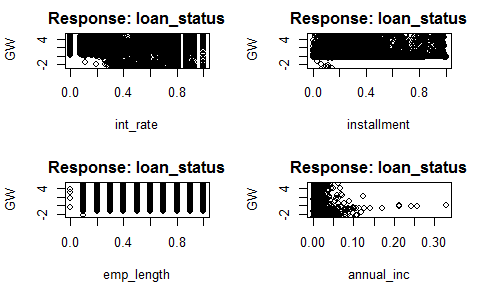
\includegraphics[width=0.8\textwidth]{image4.png}
\caption{Generalised weights of the input}
\label{fig:gw}
\end{figure}
In figure \ref{fig:gw}, generalised weights of all the covariates are shown. Distribution has shown that all the attributes have non linear effect on loan\_status since all weights have generalised weight of greater than $1$. Figure \ref{table:result} shows the accuracy of the predicted values vs actual values and predicted values have been round off.\\\\
\begin{table} 
\caption{Comparison of predicted output and desired output} % title of Table 
\centering      % used for centering table 
\begin{tabular}{l|c|c}  % centered columns
\hline                      %inserts double horizontal lines 
{\bf Actual}&{\bf Prediction}&{\bf Matches}\\
%heading 
\hline                    % inserts single horizontal line 
0 & 0.0032 & True\\
0 & 0.00017 & True\\
0 & 0.0114 & True\\
1 & 0.985 & True\\
0 & 0.0060 & True\\
0 & 0.0132 & True\\
0 & 0.9704 & False\\
0 & 0.0101 & True\\
1 & 0.00128 & True\\
\hline     %inserts single line 
\end{tabular} 
\label{table:result} 
\end{table}
Last, linear regression \cite{laitinen1999predicting} have been applied to the dataset in order to compare the accuracy of both the algorithms. glm() function has been used to fit the linear regression model. For regression a probability greater than 0.5 has been assigned, if predicted values in regression is greater than $0.5$ then value is $1$ else $0$. Accuracy has been calculated by incorporating misclassification error and confusion matrix has also calculated as shown in figure \ref{fig:image5}.\\
\begin{figure}[!htb]
\centering
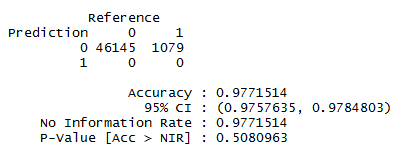
\includegraphics[width=0.8\textwidth]{image5.png}
\caption{Confusion matrix and statistics of linear regression}
\label{fig:image5}
\end{figure}
To highlight the comparison, mean square error of both linear regression and neural network has been calculated as shown in table \ref{table:mse}. As can be seen in the table mean square error of both the process are approximately same and thus both the process are doing same work. It is important to note that deviation in MSE depends on the training and test split.  
\begin{table} 
\caption{Mean Square error of both the processes} % title of Table 
\centering      % used for centering table 
\begin{tabular}{l|c}  % centered columns
\hline                      %inserts double horizontal lines 
{\bf MSE neural network}&{\bf MSE linear regression}\\
%heading 
\hline                    % inserts single horizontal line 
0.0220449 & 0.0227334\\
\hline     %inserts single line 
\end{tabular} 
\label{table:mse} 
\end{table}
\section{Conclusion and Future Work}
This paper has studied artificial neural network and linear regression models to predict credit default. Both the system has been trained on the loan lending data provided by kaggle.com. Results of both the system has shown equal effect on the dataset and thus are very effective with accuracy of $\textbf{97.67575\%}$ by artificial neural network and $\textbf{97.69609\%}$. System classifies the output variable correctly with very low error. So, both process can be used to identify credit default with equal accuracy. Also, neural network represents a black box method such that it is difficult to explain the outcome compared to linear regression model. Therefore, which model to use depends on the application one has to use. Moreover, while fitting a model using neural network process user needs to take extra care of the attributes and data normalisation to improve the performance. To conclude, neural network provides strong evidences to efficiently predict the credit default for a loan application.\\\\
Neural network algorithms have a wide range of applications that are not only essential for residential mortgages. Other applications can be rating bonds issued by companies commonly known as bond rating, rating short term investments that can last up to 1 year, long-term and short-term ratings of local and foreign currencies, sovereign, or country ratings. The prediction system can be further enhanced to assign a credit rating to an application by using appropriate algorithms and technologies.

\bibliographystyle{abbrv}
\bibliography{biblio} 
\end{document}

